A standard practice in machine learning is to divide the available data into at least three subsets: a training set, a validation set, and a test set.\cite{goodfellow_deep_2016} The training set is used to update the model parameters during optimization. The validation set is instead used to monitor generalization during development and to support decisions such as hyperparameter tuning, model selection, and stopping time. Finally, the test set is reserved for the final evaluation of the model and should not influence training decisions.\cite{goodfellow_deep_2016}

The rationale behind this separation is that good performance on the training set alone is not sufficient: the model must also perform well on unseen data. The validation set therefore provides an intermediate estimate of generalization quality while the model is being developed, whereas the test set is used only after the design choices have been fixed.\cite{goodfellow_deep_2016} In practical applications, the exact proportions assigned to these subsets depend on the size and structure of the dataset, and there is no universally optimal split.\cite{sklearn_train_test_split_2026} However, the underlying principle remains the same: parameter learning should be performed on one subset, model selection on another, and final assessment on a third independent subset. This approach helps to prevent overfitting to the training data and ensures that the reported performance metrics reflect the model's ability to generalize to new, unseen examples.\cite{goodfellow_deep_2016}
\begin{figure}[h]
    \centering
    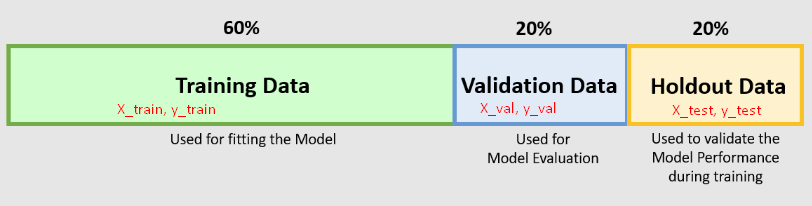
\includegraphics[width=0.85\linewidth]{images/dataset_split.png}
    \caption{Illustration of the standard partition of a dataset into training, validation, and test subsets.}
    \label{fig:dataset_split}
\end{figure}
